\section{Résultats}

Les différentes méthodes ont été testé en faisant réaliser à un essaim de 4 robots le même parcours, à savoir un carré en partant d'une position initiale fixée.
Un échantillon de résultat pour la méthode classique est donnée ci-dessous à titre d'exemple. Les robots doivent maintenir 50cm d'inter-distance avec leurs voisins, en formant une formation carré. Deux robots sont considérés comme voisins s'ils sont adjacents et forment un côté du carré. Une perturbation est également créée en déplaçant un robot à la main durant l'expérience.

\begin{figure}[H]
    \centering
    \begin{minipage}{0.48\textwidth}
        \centering
        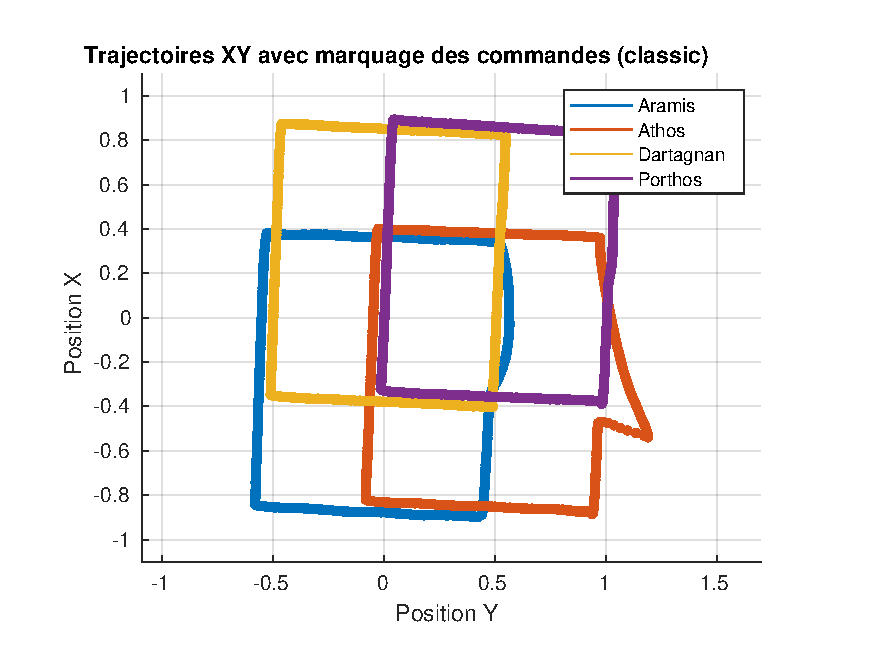
\includegraphics[width=\textwidth]{4-Resultat/pic/trajectoires_marquage.pdf}
        \caption{Trajectoire des robots avec une perturbation}
        \label{fig:essaim_trajectory2_perturbation}
    \end{minipage}\hfill
    \begin{minipage}{0.48\textwidth}
        \centering
        
\includegraphics[width=\textwidth]{4-Resultat/pic/distance.pdf}
        \caption{Evolution des inter-distances entre les robots avec perturbation}
        \label{fig:inter_distances_classic_perturbation}
    \end{minipage}
    \vspace{-0.3cm}
\end{figure}
\noindent Voici un tableau récapitulatif des résultats obtenus durant ce stage :
\begin{table}[H]
    \vspace{-0.2cm}
    \centering
    \caption{Tableau récapitulatif des performances par méthode}
    \vspace{-0.2cm}
    \label{tab:comparaison-methodes}
    \begin{tabular}{|l|c|c|c|}
        \hline
        Critère & Classique & Événementielle & Prédictive \\
        \hline
        Temps de parcours [s] & 48 & 39 & 56 \\
        Temps de convergence [s] & 13 & 26 & 15 \\
        \hline
        Nombre total de commandes calculées  & 1932 & 442 & 2187 \\
        Calculs de commande par seconde & $\approx$ 40.3 & $\approx$ 11.3 & $\approx$ 39.1 \\
        \hline
        Nombre total d'échanges de données  & 966 & 780 & 110 \\
        Échanges de données par seconde & $\approx$ 20.1 & 20 & $\approx$ 1.96 \\
        \hline
        Utilisation du processeur [\%] & $\approx$ 20 & $\approx$ 20 & $\approx$ 15 \\
        Utilisation de la mémoire vive [Mo] & $\approx$ 470 & $\approx$ 470 & $\approx$ 470 \\
        \hline
    \end{tabular}
    \vspace{-0.2cm}
\end{table}

En conclusion, les résultats obtenus sont satisfaisants et chaque méthode a répondu à ses objectifs principaux.

La méthode prédictive a réduit considérablement le nombre d'échanges de données tout en maintenant des performances de suivi de trajectoire similaires à la méthode classique. De plus, elle a permis de diminuer la charge CPU. L'intérêt de cette méthode est donc prouvé, particulièrement dans le contexte d'un essaim de grande taille. En effet, la réduction des communications est cruciale pour le passage à l'échelle : elle limite la surchage du réseau, réduisant ainsi le risque de problèmes lié au réseau.

La méthode événementielle a quant à elle bien réduit le nombre de calculs de commande. Cependant, l'intérêt de cette approche est plus discutable, car la charge CPU n'a pas diminué par rapport à la méthode classique. Pour évaluer un potentiel gain, il aurait été pertinent de mesurer la consommation énergétique des moteurs. L'hypothèse serait que le maintien d'une vitesse constante plus fréquente réduirait la consommation, bien que les accélérations brusques lors des mises à jour de commande puissent avoir l'effet inverse. Malheureusement, cette mesure n'a pas été possible durant le stage, faute de capteurs de courant.

La prochaine étape du projet consistera à transposer ces algorithmes sur des drones quadricoptères, en s'appuyant sur les enseignements tirés de cette phase expérimentale avec les robots terrestres holonomes.